\documentclass[a4paper,12pt]{article} % тип документа

%  Русский язык
\usepackage[T2A]{fontenc}			% кодировка
\usepackage[utf8]{inputenc}			% кодировка исходного текста
\usepackage[english,russian]{babel}	% локализация и переносы

\usepackage{graphicx}               % импорт изображений
\usepackage{wrapfig}                % обтекаемые изображения
\graphicspath{{pictures/}}          % обращение к подкаталогу с изображениями
\usepackage[14pt]{extsizes}         % для того чтобы задать нестандартный 14-ый размер шрифта
\usepackage{amsfonts}               % буквы с двойными штрихами
\usepackage[warn]{mathtext}         % русский язык в формулах
\usepackage{indentfirst}            % indent first
\usepackage[margin = 25mm]{geometry}% отступы полей
\usepackage{amsmath}                % можно выводить фигурные скобочки -- делать системы уравнений
\usepackage[table,xcdraw]{xcolor}   % таблицы
\usepackage{amsmath,amsfonts,amssymb,amsthm,mathtools} % Математика
\usepackage{wasysym}                % ???
\usepackage{upgreek}                % ???  
\usepackage{caption}
\captionsetup{labelsep=period}
\usepackage{gensymb} % degree symbol
\usepackage{mathrsfs}
\usepackage{multirow}

\begin{document}
	\begin{center}
		
		\textbf{НАЦИОНАЛЬНЫЙ ИССЛЕДОВАТЕЛЬСКИЙ УНИВЕРСИТЕТ \\ <<МОСКОВСКИЙ ФИЗИКО-ТЕХНИЧЕСКИЙ ИНСТИТУТ>>}
		\vspace{13ex}
		
		\textbf{Лабораторная работа 3.4.2 \\ <<Закон Кюри-Вейсса>> }
		\vspace{60ex}
		
		\normalsize{Овсянников Михаил Александрович \\ студент группы Б01-001\\ 2 курс ФРКТ\\}
	\end{center}
	
	\vfill 
	
	\begin{center}
		г. Долгопрудный\\ 
		2021 г.
	\end{center}
	
	\thispagestyle{empty} % выключаем отображение номера для этой страницы
	
	\newpage
	
	
	
\textbf{Цель работы:} изучение температурной зависимости магнитной восприимчивости ферромагнетика выше точки Кюри.

\vspace{5mm}	
\textbf{Оборудование:} катушка самоиндукции с образцом из гадолиния, термостат, частотометр, цифровой вольтметр, $ LC$-автогенератор, термопара медь-константан.


\section*{Теоретические сведения}

При повышении температуры $Т$ возрастает дезориентирующее действие теплового движения частиц, и магнитная восприимчивость парамагнетиков убывает, в простейшем случае (в постоянном магнитном поле) - пo закону Кюри.

\begin{figure}[h!]
	\centering
	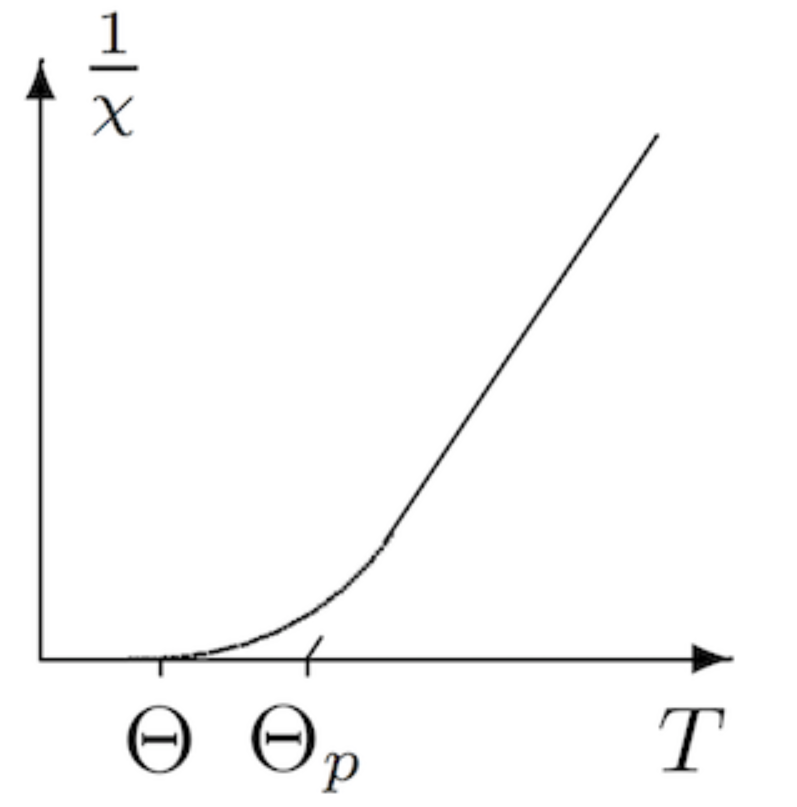
\includegraphics[scale=0.6]{Pictures/ТеорГраф.png}
	\caption{Теоретический график зависимости обратной магнитной восприимчивости от температуры}
\end{figure}

При $ T\to 0 $ тепловое движение всё меньше препятствует магнитным моментам атомов ориентироваться в одном направлении при сколь угодно слабом внешнем поле. В ферромагнетиках (под влиянием обменных сил) это происходит при понижении температуры не до абсолютного нуля, а до температуры Кюри $\Theta$, в которой добавка к температуре $\Theta_p$ --- некая температура, называемая парамагнитной точкой Кюри. Она близка к $\Theta$, но немного больше ее (см. рис.1).

В данной работе изучается температурная зависимость $ \chi(T) $ гадолиния
при температурах выше точки Кюри. Выбор материала определяется
тем, что его точка Кюри лежит в интервале комнатных температур.




\section*{Экспериментальная установка} 
\begin{figure}[h!]
	\centering
	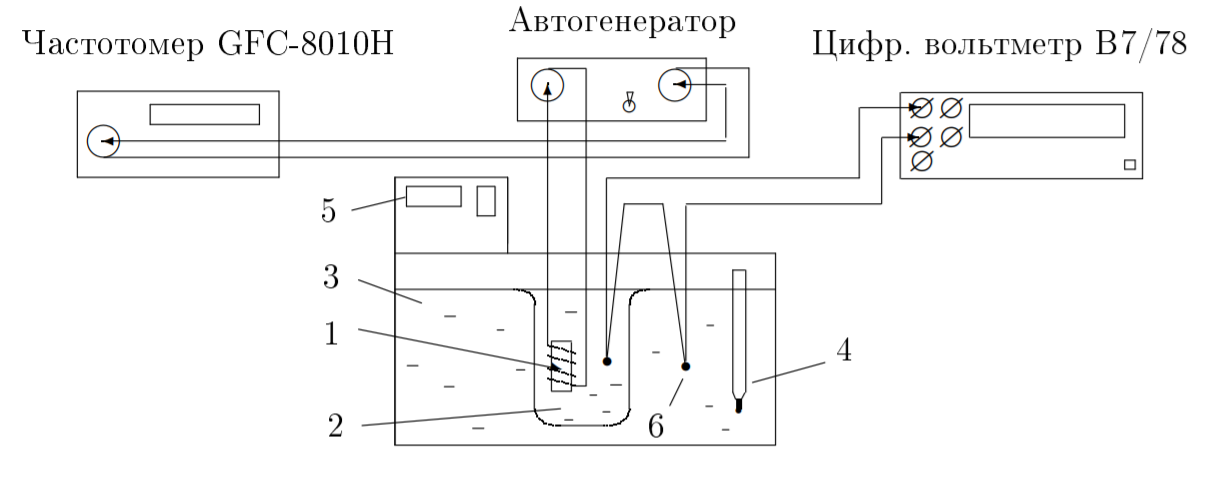
\includegraphics[scale=0.6]{Pictures/Установка.png}
	\caption{Схема экспериментальной установки}
\end{figure}

Схема установки для проверки закона Кюри-Вейсса показана на рис. 2. Исследуемый ферромагнитный образец (гадолиний) расположен внутри пустотелой катушки самоиндукции, которая служит индуктивностью колебательного контура, входящего в состав $LC$-автогенератора. 

Гадолиний является хорошим проводником электрического тока, а рабочая частота генератора достаточно велика ($\thicksim$50 кГц), поэтому для уменьшения вихревых токов образец из готовлен из мелких кусочков размером 0,5 мм. Катушка 1 с образцом помещена в стеклянный сосуд 2, залитый трансформаторным маслом. Масло предохраняет образец от окисления и способствует ухудшению электрического контакта между отдельными частичками образца. Кроме того, оно улучшает тепловой контакт между образцом и термостатируемой (рабочей) жидкостью 3 в термостате. Ртутный термометр 4 используется для приближенной оценки температуры.


При изменении температуры меняется магнитная восприимчивость образца $ \chi $, а следовательно, самоиндукция катушки и период колебаний $ \tau $ автогенератора. Для измерения периода используется частотомер.

Закон Кюри- Вейсса справедлив, если выполнено соотношение

\begin{equation}\label{}
	\dfrac{1}{\chi} \sim T - \Theta_p \sim \dfrac{1}{\tau^2 - \tau^2_0}
\end{equation}
где $ \tau_0 $ --- период колебаний без образца. 

Для нагрева используется термостат. Температура исследуемого образца всегда несколько отличается от температуры дистиллированной воды в сосуде. После того как вода достигла заданной температуры, идет медленный процесс выравнивания температур образца и воды. Разность их температур контролируется с помощью медно-константановой термопары 6 и цифрового вольтметра. Один из спаев термопары находится в тепловом контакте с образцом, а другой погружен в воду. Концы термопары подключены к цифровому вольтметру. Рекомендуется измерять период колебаний автогенератора в тот момент, когда указанная разность температур становится $  \leqslant 0,5 \;^\circ C $. Чувствительность термопары $ \kappa = 24 $ град/мВ.



\section*{Ход работы}

Запишем период колебаний $\tau_0$ без образца: $\tau_0 = 9,045$ мкс.

\vspace{5mm}
Индуктивность цепи будет вычисляться по формуле: $L = \dfrac{\mu_0 \mu N^2 S}{2\pi R}$

\vspace{3mm}
Запишем индуктивность катушки без образа: $L_0 = 1602$ мкГн.

Знаем соотношение: $\dfrac{\tau^2 - \tau_0^2}{\tau_0^2} = \mu - 1 = \chi$.

\vspace{5mm}
Снимем зависимость периода колебаний с образцом от температуры. Точность ее измерения составляет $\Delta t = 0,072$ $^\circ C$. Результаты запишем в таблицу.
	
\begin{table}[h!]
	\centering
	\begin{tabular}{|r|r|r|r|r|r|r|}
		\hline
		\multicolumn{1}{|c|}{$t$, $^\circ C$} & \multicolumn{1}{c|}{$T$, K} & \multicolumn{1}{c|}{$\tau$, мкс} & \multicolumn{1}{c|}{$\chi$} & \multicolumn{1}{c|}{$1/\chi$} & \multicolumn{1}{c|}{$\mu$} & \multicolumn{1}{c|}{$L$, мкГн} \\ \hline
		10,77                                 & 283,92                      & 10,86                            & 0,442                      & 2,263                                 & 1,442                      & 2309,9                         \\ \hline
		12,12                                 & 285,27                      & 10,84                            & 0,435                      & 2,298                                 & 1,435                      & 2299,2                         \\ \hline
		14,14                                 & 287,29                      & 10,77                            & 0,418                      & 2,395                                 & 1,418                      & 2271,0                         \\ \hline
		16,13                                 & 289,28                      & 10,66                            & 0,389                      & 2,568                                 & 1,389                      & 2226,0                         \\ \hline
		18,12                                 & 291,27                      & 10,48                            & 0,342                      & 2,923                                 & 1,342                      & 2150,1                         \\ \hline
		20,11                                 & 293,26                      & 10,17                            & 0,265                      & 3,768                                 & 1,265                      & 2027,2                         \\ \hline
		22,10                                 & 295,25                      & 9,80                             & 0,174                      & 5,759                                 & 1,174                      & 1880,2                         \\ \hline
		24,10                                 & 297,25                      & 9,52                             & 0,108                      & 9,271                                 & 1,108                      & 1774,8                         \\ \hline
		26,10                                 & 299,25                      & 9,40                             & 0,079                      & 12,628                                & 1,079                      & 1728,9                         \\ \hline
		30,09                                 & 303,24                      & 9,28                             & 0,052                      & 19,065                                & 1,052                      & 1686,0                         \\ \hline
	\end{tabular}
\caption{Данные}
\end{table}

\newpage

Теперь построим графики $\chi (T)$, $\dfrac{1}{\chi}(T)$, $\mu (T)$ и $L(T)$.

Сначала $\dfrac{1}{\chi}(T)$:

\begin{figure}[h!]
	\centering
	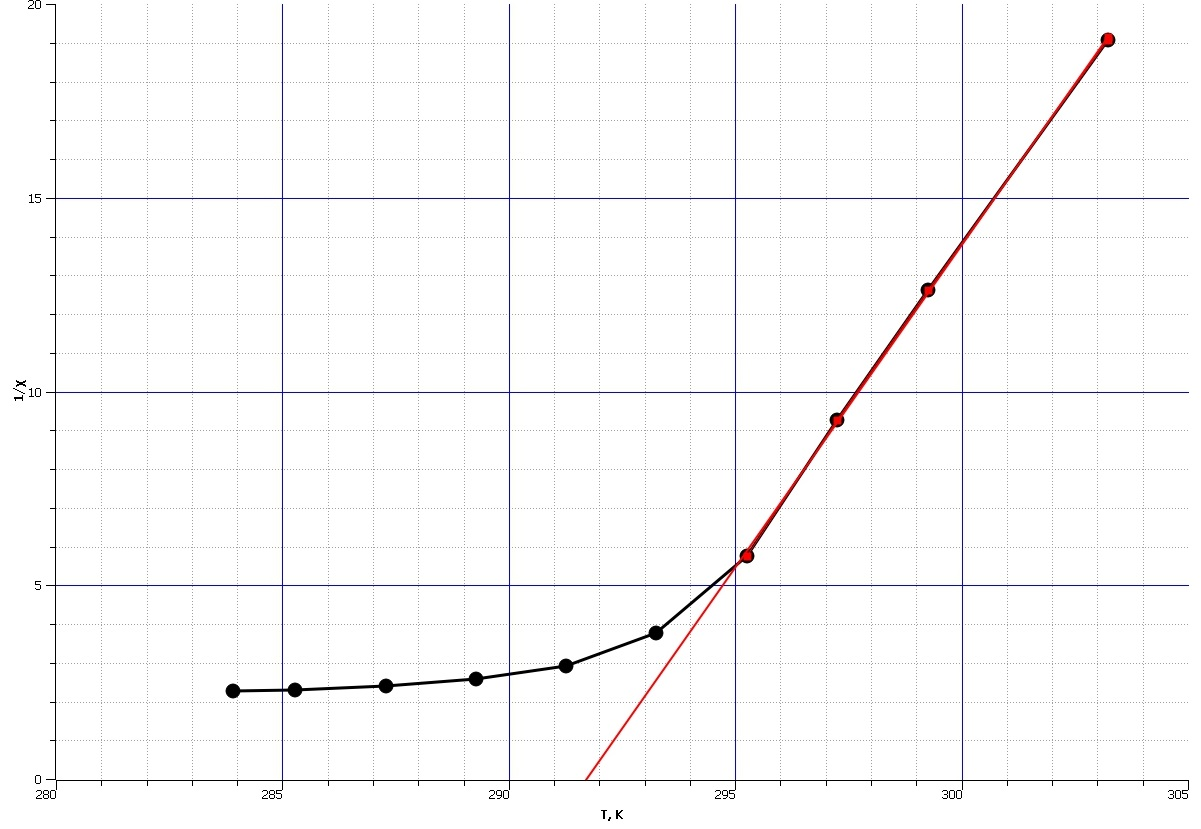
\includegraphics[scale=0.6]{Pictures/recip_chi(T).jpg}
	\caption{Зависимость $\dfrac{1}{\chi}(T) $}
\end{figure}

Из графика сразу получаем парамагнитную точку Кюри для гадолиния: $\boxed{\Theta_p = 291,7 \; \text{K}  = 18,55 \; ^\circ C}$

\newpage
Теперь $\chi (T):$

\begin{figure}[h!]
	\centering
	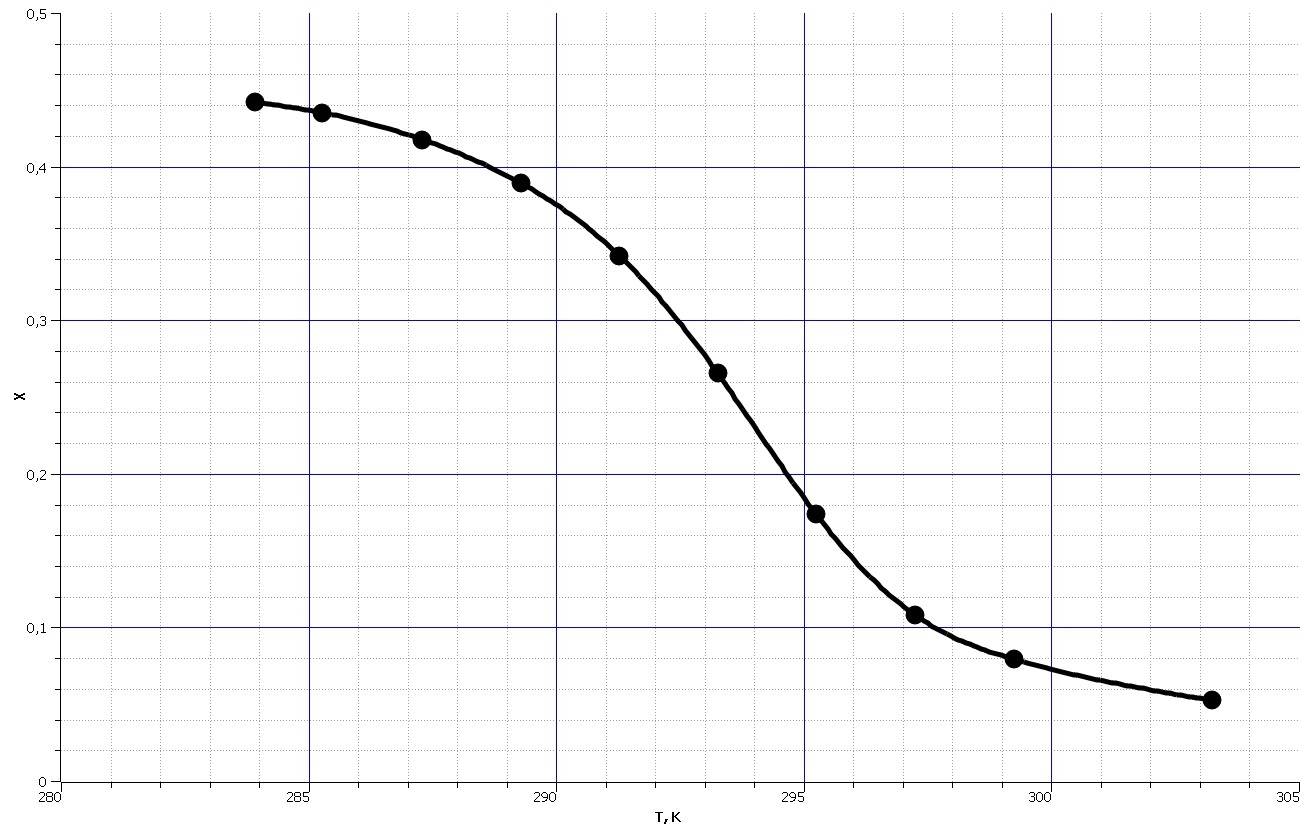
\includegraphics[scale=0.5]{Pictures/chi(T).jpg}
	\caption{Зависимость $\chi (T)$}
\end{figure}


И $\mu (T)$ и $L(T)$:

\begin{figure}[h]
\begin{minipage}[h]{0.49\linewidth}
	\centering
	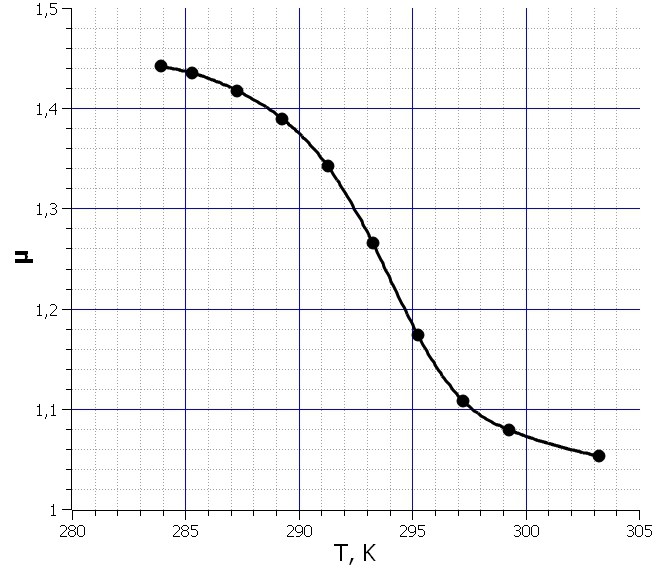
\includegraphics[scale=0.57]{Pictures/mu(T).jpg}
\end{minipage}
\hfill
\begin{minipage}[h]{0.49\linewidth}
	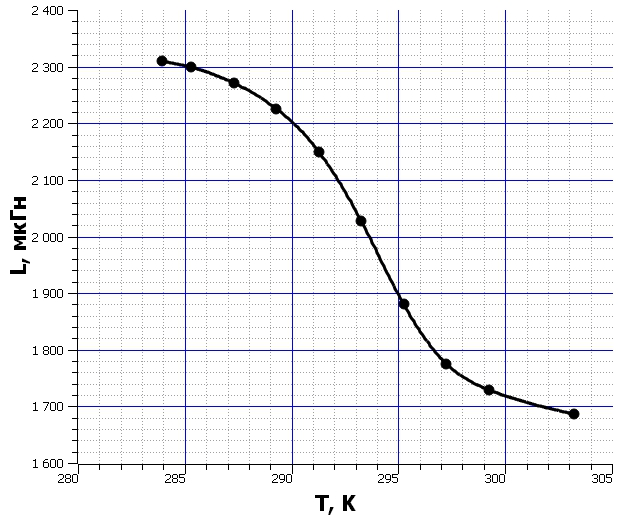
\includegraphics[scale=0.65]{Pictures/L(T).jpg}
\end{minipage}

\caption{Зависимость $\mu (T)$ и $L(T)$ соответственно}
\end{figure}

\newpage

\textbf{Вывод:} в работе была изучена температурная зависимость магнитной восприимчивости гадолиния выше точки Кюри. Была также найдена сама точка Кюри $\Theta_p = 291,7$ K. Все ошибки связаны с неточностью измерений.
\end{document}